%-----------------------------------LICENSE------------------------------------%
%   This file is part of Mathematics-and-Physics.                              %
%                                                                              %
%   Mathematics-and-Physics is free software: you can redistribute it and/or   %
%   modify it it under the terms of the GNU General Public License as          %
%   published by the Free Software Foundation, either version 3 of the         %
%   License, or (at your option) any later version.                            %
%                                                                              %
%   Mathematics-and-Physics is distributed in the hope that it will be useful, %
%   but WITHOUT ANY WARRANTY; without even the implied warranty of             %
%   MERCHANTABILITY or FITNESS FOR A PARTICULAR PURPOSE.  See the              %
%   GNU General Public License for more details.                               %
%                                                                              %
%   You should have received a copy of the GNU General Public License along    %
%   with Mathematics-and-Physics.  If not, see <https://www.gnu.org/licenses/>.%
%------------------------------------------------------------------------------%

% Use the standalone class for displaying the tikz image on a small PDF.
\documentclass[crop, tikz]{standalone}

% Needed for mathbb.
\usepackage{amssymb}

% Import the tikz package to use for the drawing.
\usepackage{tikz}

% Load the arrows.meta library.
\usetikzlibrary{arrows.meta}

% Begin the document.
\begin{document}

    % Draw the figure.
    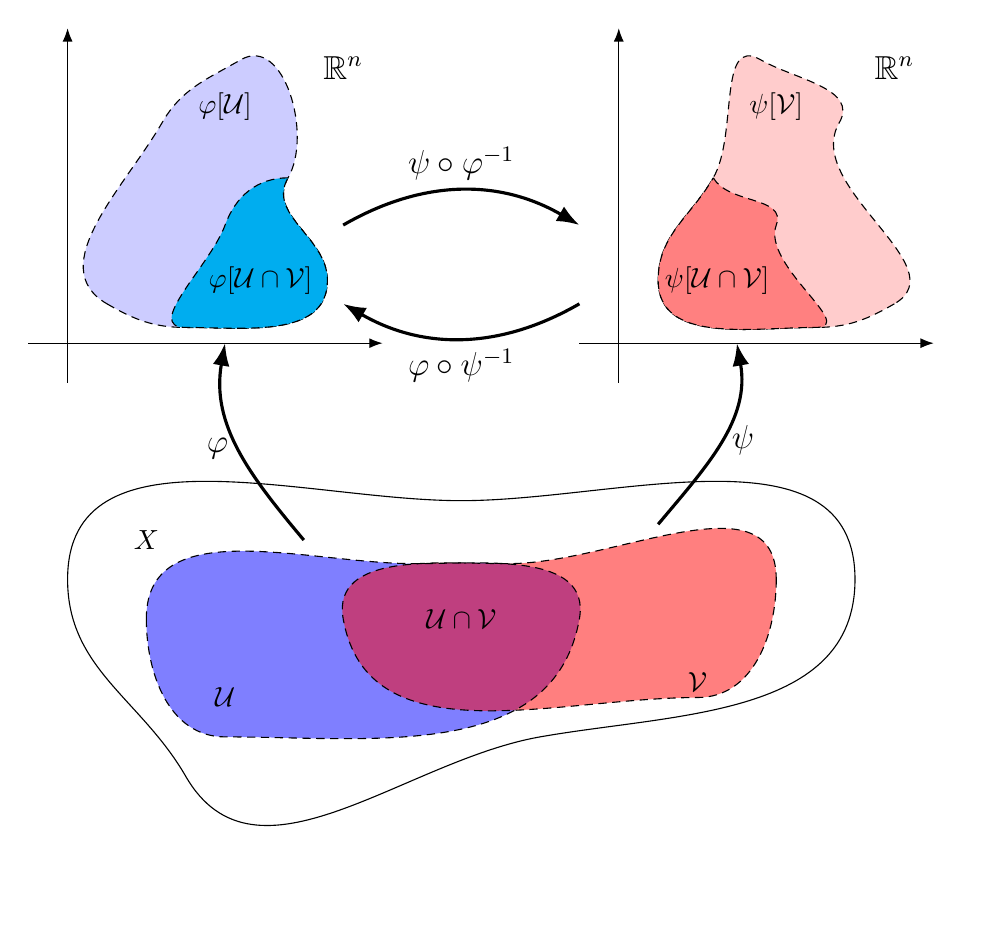
\begin{tikzpicture}[>=Latex]
        % Coordinates for the manifold X.
        \coordinate (X0) at (-5.0,  0.0);
        \coordinate (X1) at (-3.5, -2.5);
        \coordinate (X2) at ( 1.0, -2.0);
        \coordinate (X3) at ( 5.0,  0.0);
        \coordinate (X4) at ( 0.0,  1.0);

        % Coordinates for the subset U.
        \coordinate (U0) at (-4.0, -0.5);
        \coordinate (U1) at (-3.0, -2.0);
        \coordinate (U2) at ( 1.5, -0.5);
        \coordinate (U3) at (-0.6,  0.2);

        % Coordinates for the subset V.
        \coordinate (V0) at ( 4.0,  0.0);
        \coordinate (V1) at ( 3.0, -1.5);
        \coordinate (V2) at (-1.5, -0.5);
        \coordinate (V3) at ( 0.6,  0.2);

        % Draw the manifold X.
        \draw   (X0) to[out=-90, in=120]  (X1)
                     to[out=-60, in=-170] (X2)
                     to[out=10, in=-90]   (X3)
                     to[out=90, in=0]     (X4)
                     to[out=-180, in=90]  cycle;

        % Fill in U and V first and then outline with dashes.
        % This prevents the fill option from drawing over the outline.
        % Setting opacity makes the overlapping part mix colors as well.

        % Fill in the background of U blue.
        \draw[fill=blue, opacity=0.5, draw=none]
            (U0) to[out=-90, in=-180] (U1)
                 to[out=0, in=-100]   (U2)
                 to[out=80, in=0]     (U3)
                 to[out=-180, in=90]  cycle;

        % Fill in the background of V red.
        \draw[fill=red, opacity=0.5, draw=none]
            (V0) to[out=-90, in=0]   (V1)
                 to[out=180, in=-80] (V2)
                 to[out=100, in=180] (V3)
                 to[out=0, in=90]    cycle;

        % Draw dashed lines around U.
        \draw[densely dashed]
            (U0) to[out=-90, in=-180] (U1)
                 to[out=0, in=-100]   (U2)
                 to[out=80, in=0]     (U3)
                 to[out=-180, in=90]  cycle;

        \draw[densely dashed]
            (V0) to[out=-90, in=0]   (V1)
                 to[out=180, in=-80] (V2)
                 to[out=100, in=180] (V3)
                 to[out=0, in=90]    cycle;

        \begin{scope}[xshift=-5cm, yshift=3cm]

            % Coordinates for phi of U.
            \coordinate (P0) at (0.5, 0.5);
            \coordinate (P1) at (1.5, 0.2);
            \coordinate (P2) at (3.3, 0.8);
            \coordinate (P3) at (2.8, 2.1);
            \coordinate (P4) at (2.2, 3.6);
            \coordinate (P5) at (1.2, 2.8);

            % Coordinate for some midpoint inside U.
            \coordinate (PM) at (2.0, 1.5);

            \draw[->] (-0.5,  0.0) to ( 4.0,  0.0);
            \draw[->] ( 0.0, -0.5) to ( 0.0,  4.0);

            \draw[draw=none, fill=blue!20!white]
                (P0)    to[out=-30,  in=180]    (P1)
                        to[out=0,    in=-90]    (P2)
                        to[out=90,   in=-120]   (P3)
                        to[out=60,   in=30]     (P4)
                        to[out=-150, in=60]     (P5)
                        to[out=-120, in=150]    cycle;

            \draw[densely dashed]
                (P0)    to[out=-30,  in=180]    (P1)
                        to[out=0,    in=-90]    (P2)
                        to[out=90,   in=-120]   (P3)
                        to[out=60,   in=30]     (P4)
                        to[out=-150, in=60]     (P5)
                        to[out=-120, in=150]    cycle;

            \draw[densely dashed, fill=cyan]
                (P3)    to[out=180,  in=70]   (PM)
                        to[out=-110, in=180]  (P1)
                        to[out=0,    in=-90]  (P2)
                        to[out=90,   in=-120] cycle;

            \node at (2.00, 3.0) {$\varphi[\mathcal{U}]$};
            \node at (2.45, 0.8) {$\varphi[\mathcal{U}\cap\mathcal{V}]$};
            \node at (3.50, 3.5) {\large{$\mathbb{R}^{n}$}};
        \end{scope}

        \begin{scope}[xshift=2cm, yshift=3cm]

            % Coordinates for phi of U.
            \coordinate (Q0) at (3.5, 0.5);
            \coordinate (Q1) at (2.5, 0.2);
            \coordinate (Q2) at (0.5, 0.8);
            \coordinate (Q3) at (1.2, 2.1);
            \coordinate (Q4) at (1.8, 3.6);
            \coordinate (Q5) at (2.8, 2.8);

            % Coordinate for some midpoint inside U.
            \coordinate (QM) at (2.0, 1.5);

            \draw[->] (-0.5,  0.0) to ( 4.0,  0.0);
            \draw[->] ( 0.0, -0.5) to ( 0.0,  4.0);

            \draw[draw=none, fill=red!20!white]
                (Q0)    to[out=-150,    in=0]       (Q1)
                        to[out=-180,    in=-90]     (Q2)
                        to[out=90,      in=-120]    (Q3)
                        to[out=60,      in=150]     (Q4)
                        to[out=-30,     in=60]      (Q5)
                        to[out=-120,    in=30]      cycle;

            \draw[densely dashed]
                (Q0)    to[out=-150,    in=0]       (Q1)
                        to[out=-180,    in=-90]     (Q2)
                        to[out=90,      in=-120]    (Q3)
                        to[out=60,      in=150]     (Q4)
                        to[out=-30,     in=60]      (Q5)
                        to[out=-120,    in=30]      cycle;

            \draw[densely dashed, fill=red!50!white]
                (Q3)    to[out=-60,     in=70]      (QM)
                        to[out=-110,    in=0]       (Q1)
                        to[out=-180,    in=-90]     (Q2)
                        to[out=90,      in=-120]    cycle;

            \node at (2.00, 3.0) {$\psi[\mathcal{V}]$};
            \node at (1.25, 0.8) {$\psi[\mathcal{U}\cap\mathcal{V}]$};
            \node at (3.50, 3.5) {\large{$\mathbb{R}^{n}$}};
        \end{scope}

        \begin{scope}[line width=0.4mm, ->, font=\large]
            \draw (-2.0, 0.5) to[out=130, in=-100] node[left]  {$\varphi$} (-3.0, 3);
            \draw ( 2.5, 0.7) to[out=50,  in=-80]  node[right] {$\psi$}  ( 3.5, 3);
            \draw (-1.5, 4.5) to[out=30, in=150]
                node[above] {$\psi\circ\varphi^{-1}$} ( 1.5, 4.5);
            \draw ( 1.5, 3.5) to[out=-150, in=-30]
                node[below] {$\varphi\circ\psi^{-1}$} (-1.5, 3.5);
        \end{scope}

        \node at (-4.0,  0.5) {$X$};
        \node at (-3.0, -1.5) {$\mathcal{U}$};
        \node at ( 3.0, -1.3) {$\mathcal{V}$};
        \node at ( 0.0, -0.5) {$\mathcal{U}\cap\mathcal{V}$};
    \end{tikzpicture}
\end{document}
